\documentclass[tikz,border=2mm]{standalone}

\usepackage{pgfplots}  %Axis se define aqui
\usetikzlibrary{arrows.meta}
\usetikzlibrary{datavisualization.formats.functions}

\begin{document}

\begin{tikzpicture}
\begin{axis}[axis lines=middle, ymax=1.1, clip=false]
\addplot[domain=-10:10 ,samples=50, smooth] {sin(deg(x))/x};
\end{axis}
\end{tikzpicture}
%
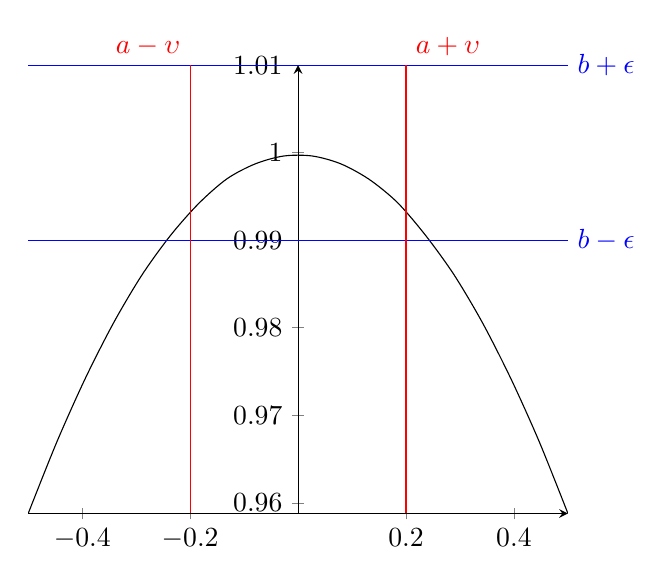
\begin{tikzpicture}
\begin{axis}[axis lines=middle,name=border, ymax=1.01, smooth]
\addplot[domain=-.5:.5 ,samples=20] {sin(deg(x))/x};
\coordinate (A) at (axis cs: -0.2,.99);
\coordinate (B) at (axis cs: 0.2,1.01);
\end{axis}
\draw[blue] (border.west |- A) -- (border.east |- A) node[right] {$b-\epsilon$};
\draw[blue] (border.west |- B) -- (border.east |- B) node[right] {$b+\epsilon$};
\draw[red] (border.south -| A) -- (border.north -| A) node[above left] {$a-\upsilon$};
\draw[red] (border.south -| B) -- (border.north -| B) node[above right] {$a+\upsilon$};
\end{tikzpicture}

\end{document}
